\section{Criterios de asignación}

\econ{https://www.core-econ.org/the-economy/book/es/text/05.html}{5}

\subsection{Criterios de asignación}
Se entiende una asignación como el resultado de un determinado proceso económico.

\subsection{Eficiencia de Pareto}
Sean $A$ y $B$ asignaciones, la eficiencia de pareto establece que:
\hfill \break
\hfill \break
\textit{La asignación $A$ prevalece sobre la asignación $B$, si al menos una de las partes estaría mejor con $A$ que con $B$, y nadie estaría peor. En este caso $A$ domina a $B$ en términos de Pareto.}
\hfill \break


Una asignación que no está dominada en términos de Pareto se denomina \textbf{Pareto-eficiente.}


Este criterio es lo que en matemáticas se conoce como un orden parcial. Es decir, permite ordenar algunas asignaciones, pero no todas (esto sería un orden completo).

\subsubsection{Comentarios sobre la eficiencia de Pareto}
El criterio de la eficiencia de Pareto es uno de los conceptos más relevantes en economía. 


Dado un problema determinado, pueden existir muchas asignaciones que son pareto-eficientes. Pero sin un criterio adicional, no podemos decir cual de ellas es preferible.


Que una asignación sea eficiente de Pareto, no significa que estemos de acuerdo con ella. De hecho, si se le entregara todo el ingreso a una persona en la sociedad y dejamos a todo el resto sin nada, esa asignación es Pareto-Eficiente, pero probablemente no estemos de acuerdo en que sea una buena asignación económica.


Además, en muchas ocasiones, existe más de una asignación eficiente en términos de Pareto.

\subsection{Asignaciones}
Existen distintos casos posibles, y según este la manera de calcular asignación óptima varía.


\href{https://www.youtube.com/watch?v=jWcbHlTCPnQ}{Video EOL}
\begin{enumerate}[label=\Roman*.]
    \item \textbf{La persona genera el bien por si misma} \textit{(\href{https://youtu.be/jWcbHlTCPnQ?t=64}{Min 1:04})}, aquí $TMS = TMT$ es la condición de asignación óptima. 
    
    \item \textbf{Coerción} \textit{(\href{https://youtu.be/jWcbHlTCPnQ?t=181}{Min 3:01})}: alguien obliga a la persona a trabajar y se queda con los excedentes luego de darle lo mínimo que necesita la persona para subsistir (esclavitud). Existe una \textit{restricción de supervivencia biológica (RSB)}.
    
    El coerzor escogerá el punto donde la distancia entre la frontera del conjunto factible y la curva de RSB sea mayor.\\
    
    $TMB = TMT$ es la asignación óptima. (TMB es la tasa relacionada con RSB)
    
    \item \textbf{Propiedad privada} \textit{(\href{https://youtu.be/jWcbHlTCPnQ?t=333}{Min 5:33})}: La otra persona tiene todo el poder de negociación pero la primera persona solo trabajará si obtiene ganancias. \\
    
    Alguien externo (e.g. Estado o familia) ofrece una producción de sobrevivencia.\\
    
    Existe una curva de indiferencia de la primera persona. Se busca maximizar la distancia entre esa curva y la frontera factible.\\
    
    $TMT = TMS$ es la condición de optimalidad.
    
    \item \textbf{Negociación colectiva} \textit{(\href{https://youtu.be/jWcbHlTCPnQ?t=510}{Min 8:30})}: La primera persona busca parte del excedente.\\
    
    Una \hyperlink{institucion}{institución} externa (e.g. Estado) establece una curva de indiferencia nueva que ha de cumplirse, no necesariamente es Pareto-eficiente.\\
    
    A la persona se le puede ofrecer una nueva curva de indiferencia que le deje con igual igual utilidad (y que cumpla lo propuesto por el Estado) o que deje a ambas partes mejor.\\
    
    $TMT = TMS$ es la condición de optimalidad.
\end{enumerate}

\subsection{Desigualdad (criterios)}
Existen distintos tipos de medida a la hora de medir desigualdad, entre estas están

\begin{itemize}
    \item \textbf{Desigualdad absoluta}: es la resta de ingresos. Posee un problema que es que posee unidades dimensionales de ingreso lo cual hace difícil comparar entre lugares que no poseen las mismas unidades monetarias. Además aumenta cuando el país crece, aunque ambos ingresos crezcan a la misma \textit{tasa}. $\quad DA = Y_R - Y_P$
    
    \item \textbf{Desigualdad relativa}: es la división entre los ingresos. Es adimensional y no aumenta trivialmente cuando el país crece. $\quad DR = Y_R/Y_P$
\end{itemize}

Por esto es preferible hacer uso de la desigualdad relativa.

\subsubsection{Razones o \textit{ratios} de desigualdad}
Es la medida más sencilla de desigualdad, es la razón entre los ingresos de los sectores más ricos y pobres de la sociedad.

\begin{itemize}
    \item Razones entre quintiles
    \item Razones entre deciles
\end{itemize}

\subsubsection{Razón o índice de Palma}
Es un refinamiento de los \textit{ratios}, este índice considera que hay 3 grupos en la sociedad
\begin{enumerate}[label=\arabic*)]
    \item Los ricos (decil 10)
    \item Clase media (Decil 5 a 9)
    \item Los pobres (Decil 1 a 4)
\end{enumerate}

Se sustenta con la observación empírica: la clase media tiende a capturar la mitad del ingreso. 

\[\text{Razón de palma} = \frac{D_{10}}{D_1+D_2+D_3+D_4}\]

\subsubsection{Coeficiente o índice de Gini}
Es la medida más usada de desigualdad, representa que tanto se aleja una distribución real de una distribución totalmente igualitaria. Su valor varía entre 0 y 1, siendo mínima la desigualdad en 0 y máxima en 1. Posee dos formas:

\begin{enumerate}[label=\roman*.]
    \item \textbf{Forma general}: promedio de las diferencias de ingreso entre todos los individuos en una economía. Se calcula como \newline
    \[G = \frac{\sum_i\sum_j\abs{y_i-y_j}}{2\sum_{ij}y_i}\]
    
    \item \textbf{Forma de Sen}: suma ponderada de ingresos. (más usada)
    \newline
    \[G = \frac{2}{n}\frac{\sum_i^n i y_i}{\sum_i^n y_i} - \frac{n+1}{n}\]
\end{enumerate}


Donde $y_i$ son los ingresos correspondientes a $i$, e $i$ pueden ser deciles, quintiles, personas, etc. de las que hay una cantidad $n$.
\\

La interpretación más usual del coeficiente de Gini es a partir de la curva de Lorenz.
\subsubsection{Curva de Lorenz}
Muestra los ingresos acumulados desde los individuos más pobres a los más ricos de la sociedad. Comparándolos con la curva correspondiente a una distribución perfectamente igualitaria (DPI).

\begin{figure}[H]
    \centering
    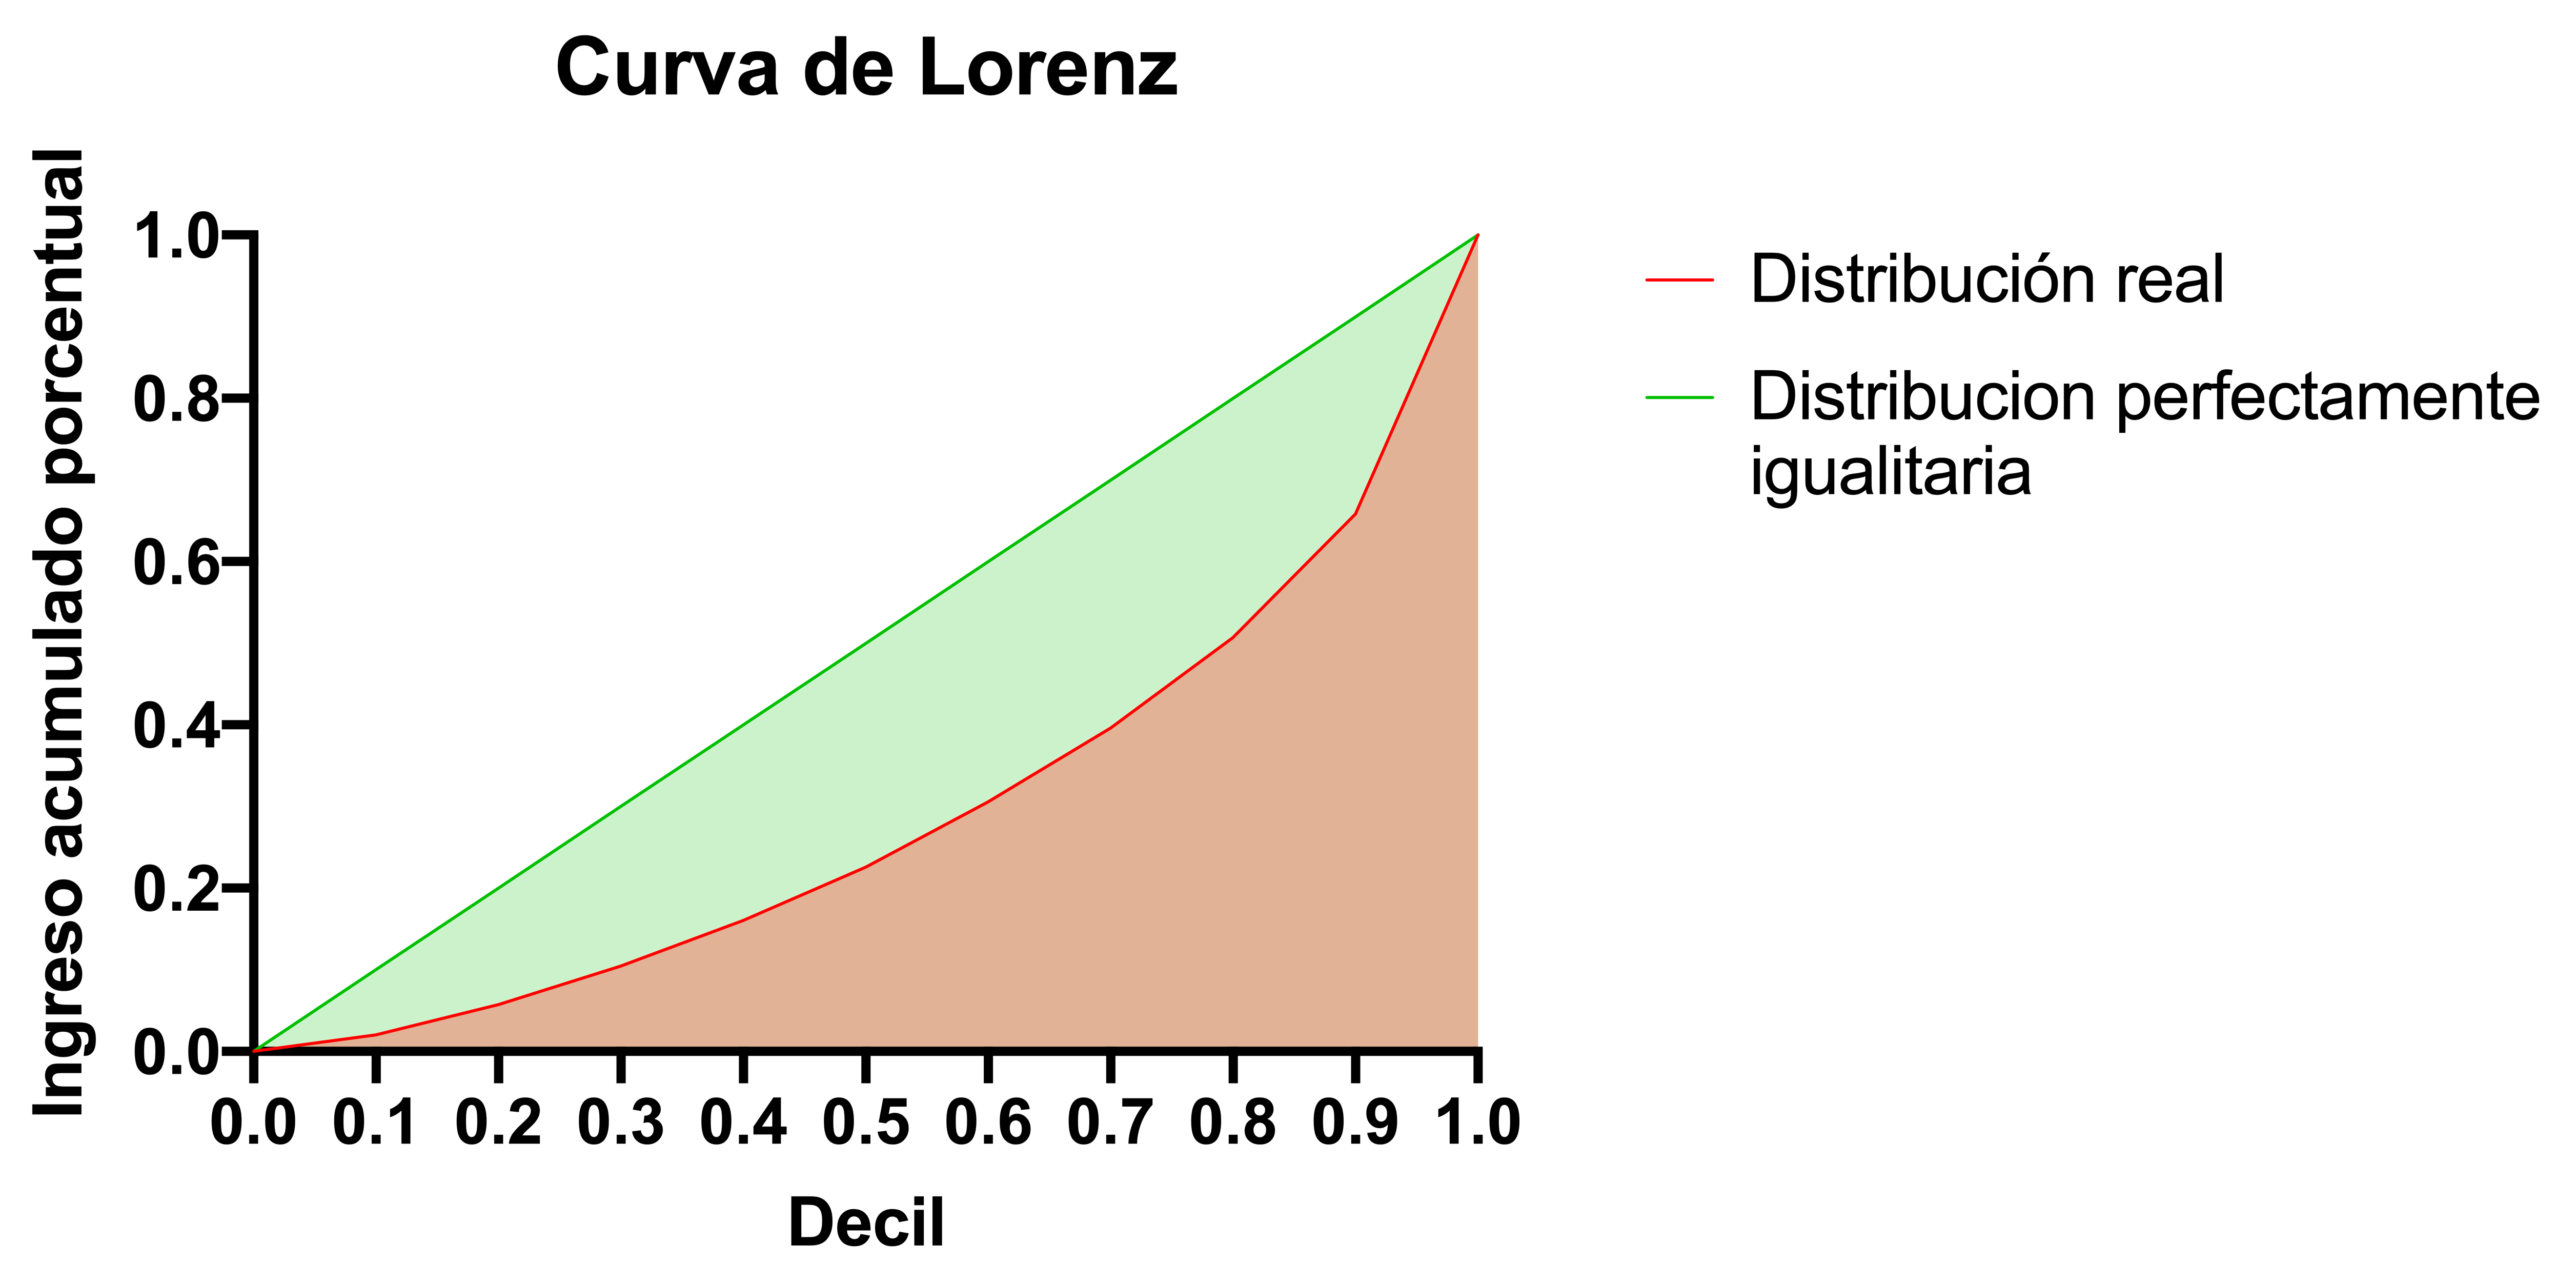
\includegraphics[width=0.84\textwidth]{Modulo_4/Curva_Lorenz_Final.png}
    \caption{Curva de Lorenz correspondiente a Chile, Casen 2017}
    \label{fig:lorenz_casen_2017}
\end{figure}

La figura \ref{fig:lorenz_casen_2017} muestra la curva de Lorenz correspondiente a Chile según la encuesta Casen 2017. En esta se puede observar en el eje vertical el \textit{Ingreso acumulado porcentual} y en el eje horizontal el \textit{Decil correspondiente} donde $0.1$ corresponde al decil 1, y así sucesivamente. \hfill \break


El índice de Gini se puede calcular a partir de las áreas bajo la curva del gráfico. Dividiendo el área entre la curva de la DPI y la distribución real, y sobre el área total. 
\[G = \frac{A_{DPI} - A_{DR}}{A_{total}}\]


En el caso de la figura \ref{fig:lorenz_casen_2017}, correspondería a dividir el área verde sobre la suma de las áreas verde y naranja. 
\newpage